\documentclass[a4paper, 10pt]{article}
\usepackage{scrextend}
\changefontsizes{9pt}
% Per-subject config for this repo. See vendor/template/course-config.tex.example
% for what each macro is used for.

\newcommand{\CourseCode}{2110413}
\newcommand{\CourseName}{Computer Security}
\newcommand{\StudentID}{6733172621}
\newcommand{\StudentName}{Patthadon Phengpinij}
\newcommand{\DefaultCollaborators}{Claude (for\,\LaTeX\,styling and grammar checking)}
\newcommand{\AssignmentLabel}{Activity}

\usepackage{../vendor/template/CEDT-Assignment-style}

\begin{document}
\subject
\asgntitle{5}{}{Public Key Infrastructure}{\StudentID\ \StudentName}{\DefaultCollaborators}

% ================================================================================ %
\section*{Overview}
% ================================================================================ %

In this activity, you will learn the fundamentals of Public Key Infrastructure.
We will need the following tools:
\begin{enumerate}[label=\Alph*.]
	\item OpenSSL. On Linux and Mac OS X, the OpenSSL is installed by default.
				For Windows, you may download it from
				\href{https://wiki.openssl.org/index.php/Binaries}{https://wiki.openssl.org/index.php/Binaries}.
	\item Python with PyOpenSSL and pem to do our exercise.
				If you python does not come with PyOpenSSL and pem, you may install it with pip
				\begin{codingbox}[language=bash]
$ pip install pyopenssl
$ pip install pem
\end{codingbox}
	\item You also need ca-certificates.crt from your OS (e.g. \texttt{/etc/cacerts/ca-certificates.crt} in Linux)
  			or take it from the course web.
\end{enumerate}

% ================================================================================ %
\section*{Exercise}
% ================================================================================ %

Issuing the following command.
\begin{codingbox}[language=bash]
$ openssl s_client -connect www.chula.ac.th:443
$
\end{codingbox}

\noindent Once connected, you may try
\begin{codingbox}[language=bash]
GET / HTTP/1.0
[Enter twice]
\end{codingbox}

\noindent (Note that the server may return HTTP 404.
This is completely normal since we did not send a request for a valid resource.)

\noindent Repeat the same step again, now with
\begin{codingbox}[language=bash]
$ openssl s_client -connect www.chula.ac.th:443 -CAfile ca-certificates.crt
$ 
\end{codingbox}

\noindent This command basically connects to port 443 (HTTPS) with the TLS/SSL. This is like
a standard telnet command, but with openssl performing the encryption for you.

\newpage

% ================================================================================ %
%                                    Problem 01                                    %
% ================================================================================ %
\begin{problem}
From the two given openssl commands, what is the difference?
Note: If your operating system does not show any error in the first command, try
\begin{codingbox}[language=bash]
$ openssl s_client -connect www.chula.ac.th:443 -CApath empty_dir
$
\end{codingbox}
If the results are still the same, your system is not reliable.
You may ignore this exercise.
(Modern versions of Mac OS X will always read CA from keychains. There is no intuitive way to turn it off.)
\end{problem}

\begin{solution}
	\noindent \textbf{Answer:} the certificate chain is the same, but only the command with \texttt{-CAfile ca-certificates.crt} can verify it.

	\myspace

	\noindent (On Ubuntu the first command reads the system store by default and also says \texttt{ok}, so I used \texttt{-CApath empty\_dir} for it.)

	\myspace

\begin{codingbox*}[numbers=none, xleftmargin=0pt, belowskip=6pt, basicstyle=\ttfamily\footnotesize\color{editortext}]
# -CApath empty_dir  (no trusted root)
depth=2 C = GB, O = Sectigo Limited, CN = Sectigo Public Server Authentication Root R46
verify error:num=20:unable to get local issuer certificate
Verify return code: 20 (unable to get local issuer certificate)

# -CAfile ca-certificates.crt
depth=2 C = GB, O = Sectigo Limited, CN = Sectigo Public Server Authentication Root R46
depth=1 C = GB, O = Sectigo Limited, CN = Sectigo Public Server Authentication CA DV R36
depth=0 CN = *.chula.ac.th
Verify return code: 0 (ok)
\end{codingbox*}
	Both connections still work (TLS is set up and the server answers the \texttt{GET}).
	The difference is only whether the client can \textbf{trust} the server's identity.
\end{solution}
% ================================================================================ %

% ================================================================================ %
%                                    Problem 02                                    %
% ================================================================================ %
\begin{problem}
	What does the error (\textbf{\underline{verify error}}) in the first command mean?
	Please explain.
\end{problem}

\begin{solution}
	\noindent \textbf{Answer:} \texttt{unable to get local issuer certificate} means OpenSSL followed the chain up to
	\texttt{Sectigo Public Server Authentication Root R46}, but could not find a \textbf{trusted root} for it in its local store (the store is empty).

	So the chain cannot end at a CA that we trust, and the server could be anyone (e.g.\ a man-in-the-middle).
	The connection is encrypted, but the server is not authenticated.
\end{solution}
% ================================================================================ %

\newpage

% ================================================================================ %
%                                    Problem 03                                    %
% ================================================================================ %
\begin{problem}
	Copy the server certificate
	(beginning with \texttt{-----BEGIN CERTIFICATE-----} and ending with \texttt{-----END CERTIFICATE-----})
	and store it as \texttt{www\_chula\_ac\_th.cert}.
	Use the command
	\begin{codingbox}[language=bash]
$ openssl x509 -in www_chula_ac_th.cert -text
$
\end{codingbox}
	\noindent to show a text representation of the certificate content.
	Briefly explain what is stored in an X.509 certificate (i.e. data in each field).
\end{problem}

\begin{solution}
	\noindent \textbf{Answer:} an X.509 certificate binds a \textbf{public key} to an \textbf{identity}, signed by a CA.
	Main fields from \texttt{openssl x509 -in www\_chula\_ac\_th.cert -text}:
	\begin{center}
		\footnotesize
		\begin{tabular}{p{0.3\linewidth}p{0.62\linewidth}}
			\toprule
			Field & Value (www.chula.ac.th) / meaning \\
			\midrule
			Version, Serial Number & v3; a unique number given by the CA (used in revocation) \\
			Signature Algorithm & \texttt{sha256WithRSAEncryption}: how the CA signed it \\
			Issuer & \texttt{Sectigo Public Server Authentication CA DV R36}: the CA that signed it \\
			Validity & 5 Jan 2026 -- 5 Feb 2027 \\
			Subject & \texttt{CN = *.chula.ac.th}: the owner \\
			Subject Public Key Info & RSA 2048-bit public key of the server \\
			Key Usage / Extended Key Usage & Digital Signature, Key Encipherment / TLS server (and client) authentication \\
			Basic Constraints & \texttt{CA:FALSE}: cannot sign other certificates \\
			Subject Alternative Name & \texttt{*.chula.ac.th}, \texttt{chula.ac.th}: hostnames it is valid for \\
			Authority Information Access & where to get the issuer cert (\texttt{CA Issuers}) and check revocation (\texttt{OCSP}) \\
			Certificate Policies & DV policy (\texttt{2.23.140.1.2.1}): only the domain was validated \\
			CT SCTs & proof that it was logged in Certificate Transparency logs \\
			Signature Value & the CA's signature over all the fields above \\
			\bottomrule
		\end{tabular}
	\end{center}
\end{solution}
% ================================================================================ %

% ================================================================================ %
%                                    Problem 04                                    %
% ================================================================================ %
\begin{problem}
	From the information in exercise 3, is there an intermediate certificate?
	If yes, what purpose does it serve?

	\noindent \textbf{Hint:} Look for an issuer and download the intermediate certificate.
	You may use the command:
	\begin{codingbox}[language=bash]
$ openssl x509 -inform der -in intermediate.cert -text
$
\end{codingbox}
	\noindent to show the details of the intermediate certificate.
	(Note that the \texttt{-inform der} is for reading the DER file. The default file format for x509 is the PEM file.)
\end{problem}

\begin{solution}
	\noindent \textbf{Answer: yes.} The issuer of the server certificate is \texttt{Sectigo Public Server Authentication CA DV R36}, which is not a root.
	I downloaded it from the \texttt{CA Issuers} URL in the certificate:
\begin{codingbox*}[numbers=none, xleftmargin=0pt, belowskip=6pt, basicstyle=\ttfamily\footnotesize\color{editortext}]
$ curl -o intermediate.cert http://crt.sectigo.com/SectigoPublicServerAuthenticationCADVR36.crt
$ openssl x509 -inform der -in intermediate.cert -text
  Issuer:  C = GB, O = Sectigo Limited, CN = Sectigo Public Server Authentication Root R46
  Subject: C = GB, O = Sectigo Limited, CN = Sectigo Public Server Authentication CA DV R36
  X509v3 Basic Constraints: critical
      CA:TRUE, pathlen:0
  X509v3 Key Usage: critical
      Digital Signature, Certificate Sign, CRL Sign
\end{codingbox*}

	\myspace

	\noindent \textbf{Purpose:} the intermediate CA signs the end-entity (server) certificates \emph{on behalf of} the root.
	The root private key can then be kept \textbf{offline}.
	If the intermediate is compromised, only it has to be revoked, not the root that is built into every OS/browser.
	The chain is: \texttt{*.chula.ac.th} $\leftarrow$ \texttt{CA DV R36} $\leftarrow$ \texttt{Root R46} (in \texttt{ca-certificates.crt}).
\end{solution}
% ================================================================================ %

\newpage

% ================================================================================ %
%                                    Problem 05                                    %
% ================================================================================ %
\begin{problem}
	Is there an intermediate CA, i.e. is there more than one organization involved in the certification?
	Say why you think so.
\end{problem}

\begin{solution}
	\noindent \textbf{Answer: there is an intermediate CA, but it belongs to the same organization as the root.}
	Only one organization does the certification.

	The intermediate (\texttt{CA DV R36}) and the root (\texttt{Root R46}) both have \texttt{O = Sectigo Limited}.
	The intermediate is just Sectigo's own sub-CA.
	The server also sends a cross-certificate of \texttt{Root R46} signed by \texttt{USERTrust RSA Certification Authority}, but USERTrust is also owned by Sectigo.
	Chulalongkorn University is only the subject, not a CA.
\end{solution}
% ================================================================================ %

% ================================================================================ %
%                                    Problem 06                                    %
% ================================================================================ %
\begin{problem}
	What is the role of \texttt{ca-certificates.crt}?
\end{problem}

\begin{solution}
	\noindent \textbf{Answer:} it is the \textbf{trust store}, the list of root CA certificates that we trust in advance (shipped with the OS).

	A chain is accepted only if it ends at one of these roots.
	This is why \texttt{-CAfile ca-certificates.crt} gives \texttt{Verify return code: 0 (ok)} and an empty store gives error 20.
\end{solution}
% ================================================================================ %

% ================================================================================ %
%                                    Problem 07                                    %
% ================================================================================ %
\begin{problem}
	Explore the \texttt{ca-certificates.crt}.
	How many certificates are in there?
	Give the command/method you have used to count.
\end{problem}

\begin{solution}
	\noindent \textbf{Answer: 121 certificates} (\texttt{ca-certificates.crt} from Ubuntu 22.04).

	\myspace
	
	Every certificate starts with exactly one \texttt{BEGIN CERTIFICATE} line, so I count those lines:

	\myspace

\begin{codingbox*}[numbers=none, xleftmargin=0pt, belowskip=6pt, basicstyle=\ttfamily\footnotesize\color{editortext}]
$ grep -c "BEGIN CERTIFICATE" ca-certificates.crt
121
$
\end{codingbox*}
\end{solution}
% ================================================================================ %

% ================================================================================ %
%                                    Problem 08                                    %
% ================================================================================ %
\begin{problem}
	Extract a root certificate from \texttt{ca-certificates.crt}.
	Use the openssl command to explore the details.
	Do you see any Issuer information?
	Please compare it to the details of www.chula.ac.th's certificate and the details of the intermediate certificate.
\end{problem}

\begin{solution}
	\noindent \textbf{Answer: yes, it has an Issuer, but Issuer = Subject} (the root is \textbf{self-signed}).
	I split the bundle into one file per certificate and picked \texttt{Sectigo Public Server Authentication Root R46}
	(the root of the www.chula.ac.th chain):

	\myspace

	\begin{codingbox*}[numbers=none, xleftmargin=0pt, belowskip=6pt, basicstyle=\ttfamily\footnotesize\color{editortext}]
$ awk '/BEGIN CERT/{n++} n{print > ("roots/" n ".pem")}' ca-certificates.crt
$ for f in roots/*.pem; do openssl x509 -in $f -noout -subject | grep -q "Root R46$" && cp $f root_sectigo_r46.pem; done
$ openssl x509 -in root_sectigo_r46.pem -text
\end{codingbox*}

	\begin{center}
		\footnotesize
		\begin{tabular}{llll}
			\toprule
			& Server (\texttt{*.chula.ac.th}) & Intermediate (\texttt{CA DV R36}) & Root (\texttt{Root R46}) \\
			\midrule
			Issuer & CA DV R36 & Root R46 & \textbf{Root R46 (itself)} \\
			Basic Constraints & \texttt{CA:FALSE} & \texttt{CA:TRUE, pathlen:0} & \texttt{CA:TRUE} \\
			Key Usage & Digital Sig., Key Encipherment & Cert Sign, CRL Sign & Cert Sign, CRL Sign \\
			Public key & RSA 2048 & RSA 3072 & RSA 4096 \\
			Validity & about 1 year (to 2027) & 15 years (to 2036) & 25 years (to 2046) \\
			\bottomrule
		\end{tabular}
	\end{center}

	Nobody signs the root for us to check it.
	It is trusted only because it is already in the trust store.
	Going up the chain, the certificates also get bigger keys and longer lifetimes.
\end{solution}
% ================================================================================ %

% ================================================================================ %
%                                    Problem 09                                    %
% ================================================================================ %
\begin{problem}
	If the intermediate certificate is not in a PEM format (text readable), use the following
	command to convert a DER file (.crt .cer .der) to PEM file:
	\begin{codingbox}[language=bash]
$ openssl x509 -inform der -in certificate.cer -out certificate.pem
$
\end{codingbox}
	\noindent (You need the pem file for exercise 10.)
\end{problem}

\begin{solution}
	\noindent The downloaded intermediate is DER (binary), so I converted it to PEM:

	\myspace

\begin{codingbox*}[numbers=none, xleftmargin=0pt, belowskip=6pt, basicstyle=\ttfamily\footnotesize\color{editortext}]
$ openssl x509 -inform der -in intermediate.cert -out intermediate.pem
$ head -1 intermediate.pem
-----BEGIN CERTIFICATE-----
\end{codingbox*}
\end{solution}
% ================================================================================ %

% ================================================================================ %
%                                    Problem 10                                    %
% ================================================================================ %
\begin{problem}
	From the given python code\( ^{\href{http://www.yothenberg.com/validate-x509-certificate-in-python/}{[1]}} \),
	implement the certificate validation.
	\begin{codingbox*}
from OpenSSL import crypto
import pem

def verify():
	with open("./target.cert", "r") as cert_file:
		cert = cert_file.read()

	with open("./intermediate.cert", "r") as int_cert_file:
		int_cert = int_cert_file.read()

	pems = pem.parse_file("./ca-certificates.cert");
	trusted_certs = []
	for mypem in pems:
		trusted_certs.append(str(mypem));

	trusted_certs.append(int_cert);
	
	verified = verify_chain_of_trust(cert, trusted_certs)

	if verified:
		print("Certificate verified")


def verify_chain_of_trust(cert_pem, trusted_cert_pems):
	certificate = crypto.load_certificate(crypto.FILETYPE_PEM, cert_pem)
	
	# Create and fill a X509Store with trusted certs
	store = crypto.X509Store()
	for trusted_cert_pem in trusted_cert_pems:
		trusted_cert = crypto.load_certificate(crypto.FILETYPE_PEM, trusted_cert_pem)
		store.add_cert(trusted_cert)

	# Create a X509StoreContext with the cert and trusted certs
	# and verify the the chain of trust
	store_ctx = crypto.X509StoreContext(store, certificate)
	# Returns None if certificate can be validated
	result = store_ctx.verify_certificate()

	if result is None:
		return True
	else:
		return False
\end{codingbox*}
	\noindent Use your program to verify the certificates of: \\
	www.chula.ac.th, google, classdeedee.cloud.cp.eng.chula.ac.th
\end{problem}

\begin{solution}
	\noindent \textbf{Answer: all four certificates are verified.}

	\myspace

	I used the given code with two small changes.
	\begin{itemize}
		\item \texttt{verify\_certificate()} raises an exception when it fails (it does not return a value), so I catch it and print the reason.
		\item The intermediate file may contain more than one certificate (the whole chain sent by the server), so it is parsed with \texttt{pem.parse\_file} as well.
	\end{itemize}
	\texttt{get\_chain.sh} saves \texttt{<host>.cert} and \texttt{<host>\_intermediate.cert} from \texttt{openssl s\_client -showcerts}.

	\myspace

	\begin{codingbox*}[language=Python, belowskip=6pt]
def verify(target, intermediate, ca_file="./ca-certificates.crt"):
    with open(target, "r") as cert_file:
        cert = cert_file.read()
    trusted_certs = [str(mypem) for mypem in pem.parse_file(ca_file)]
    if intermediate:
        trusted_certs += [str(mypem) for mypem in pem.parse_file(intermediate)]
    return verify_chain_of_trust(cert, trusted_certs)

def verify_chain_of_trust(cert_pem, trusted_cert_pems):
    certificate = crypto.load_certificate(crypto.FILETYPE_PEM, cert_pem)
    store = crypto.X509Store()
    for trusted_cert_pem in trusted_cert_pems:
        store.add_cert(crypto.load_certificate(crypto.FILETYPE_PEM, trusted_cert_pem))
    store_ctx = crypto.X509StoreContext(store, certificate)
    try:
        store_ctx.verify_certificate()
        return True, "OK"
    except crypto.X509StoreContextError as e:
        return False, str(e)
\end{codingbox*}
\begin{codingbox*}[numbers=none, xleftmargin=0pt, belowskip=6pt, basicstyle=\ttfamily\footnotesize\color{editortext}]
$ for h in www.chula.ac.th google.com classdeedee.cloud.cp.eng.chula.ac.th; do ./get_chain.sh $h; done
$ python verify.py www.chula.ac.th google.com classdeedee.cloud.cp.eng.chula.ac.th self-signed.badssl.com
www.chula.ac.th                          Certificate verified
google.com                               Certificate verified
classdeedee.cloud.cp.eng.chula.ac.th     Certificate verified
self-signed.badssl.com                   NOT verified: self-signed certificate
www_chula_ac_th.cert + intermediate.pem  (True, 'OK')
www_chula_ac_th.cert (no intermediate)   (False, 'unable to get local issuer certificate')
$
\end{codingbox*}
	The last three lines are checks that the program can also \emph{reject}: a self-signed certificate fails, and the chula certificate fails without its intermediate.
	\textbf{Note:} this code checks only the chain of trust, not the hostname.
	\texttt{classdeedee...} is served the \texttt{*.cloud.cp.eng.chula.ac.th} certificate, which still matches through the wildcard
	(\texttt{openssl verify -verify\_hostname} also says OK).
\end{solution}
% ================================================================================ %

% ================================================================================ %
%                                    Problem 11                                    %
% ================================================================================ %
\begin{problem}
	Nowaday, there are root certificates for class 1 and class 3.
	What uses would a class 1 signed certificate have that a class 3 doesn't, and vice versa?
\end{problem}

\begin{solution}
	\noindent \textbf{Answer:} the class shows how strongly the CA checked the identity of the owner.
	\begin{itemize}
		\item \textbf{Class 1} only checks that you control the e-mail address/domain.
		      It is cheap or free and quick to get, so it is good for personal e-mail signing/encryption (S/MIME), test servers and small personal sites.
		      Class 3 is overkill for these.
		\item \textbf{Class 3} checks the real organization (documents, legal existence).
		      It is used where users must trust \emph{who} is behind the key: banks, e-commerce, government servers, code signing.
		      A Class 1 certificate gives no assurance of identity, so it cannot be used for these.
	\end{itemize}
\end{solution}
% ================================================================================ %

\newpage

% ================================================================================ %
%                                    Problem 12                                    %
% ================================================================================ %
\begin{problem}
	Assuming that a Root CA in your root store is hacked and under the control of an attacker,
	and this is not noticed by anyone for months.
	\begin{subproblems_alpha}
		\item What further attacks can the attacker stage? Draw a possible attack setup.
		\item In the attack you have described above, can we rely on CRLs or OCSP for protection? Please explain.
	\end{subproblems_alpha}
\end{problem}

\begin{solution}
	\begin{enumerate}[label=(\alph*)]
		\item \textbf{Attack:} with the root's private key the attacker can issue a \textbf{valid certificate for any domain}
		      (e.g.\ \texttt{www.chula.ac.th}, a bank, Gmail).
		      Every client that trusts this root accepts it.
		      Combined with a man-in-the-middle position (rogue Wi-Fi, ARP/DNS spoofing, BGP hijack, malicious ISP),
		      the attacker can decrypt and modify all HTTPS traffic without any browser warning.
		      They can steal passwords and session cookies or inject malware.
		      They can also sign malware/fake updates (code signing) and fake S/MIME e-mails.
		      \begin{center}
			      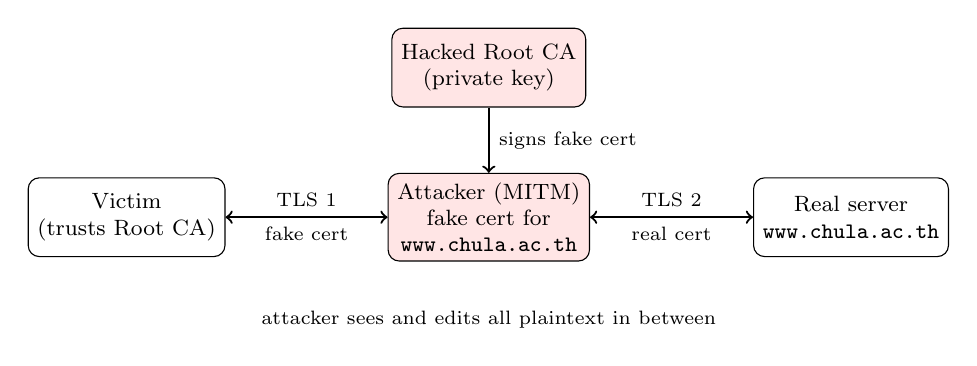
\begin{tikzpicture}[node distance=4.6cm, every node/.style={font=\footnotesize},
					      box/.style={draw, rounded corners, align=center, minimum height=1cm, minimum width=2.2cm}]
				      \node[box] (v) {Victim\\(trusts Root CA)};
				      \node[box, right of=v, fill=red!10] (m) {Attacker (MITM)\\fake cert for\\\texttt{www.chula.ac.th}};
				      \node[box, right of=m] (s) {Real server\\\texttt{www.chula.ac.th}};
				      \node[box, above of=m, node distance=1.9cm, fill=red!10] (ca) {Hacked Root CA\\(private key)};
				      \draw[->, thick] (ca) -- node[right]{\scriptsize signs fake cert} (m);
				      \draw[<->, thick] (v) -- node[above]{\scriptsize TLS 1} node[below]{\scriptsize fake cert} (m);
				      \draw[<->, thick] (m) -- node[above]{\scriptsize TLS 2} node[below]{\scriptsize real cert} (s);
				      \node[below of=m, node distance=1.3cm] {\scriptsize attacker sees and edits all plaintext in between};
			      \end{tikzpicture}
		      \end{center}
		\item \textbf{No, CRLs and OCSP do not help here.}
		      \begin{itemize}
			      \item A CRL/OCSP response is produced \textbf{by the same CA} that is compromised.
			            The attacker can sign ``good'' OCSP responses, or the CA simply does not know about the fake certificates, so they are never listed.
			      \item Nobody has noticed for months, so nothing gets revoked.
			      \item A \textbf{root cannot revoke itself}: there is no higher CA to put it on a CRL.
			            The only fix is to remove the root from every trust store (OS/browser update).
			      \item Clients often \textbf{soft-fail}: if a MITM blocks the CRL/OCSP request, browsers usually accept the certificate anyway.
		      \end{itemize}
		      Better protections are Certificate Transparency logs (fake certificates become publicly visible) and certificate pinning.
	\end{enumerate}
\end{solution}
% ================================================================================ %

\end{document}
